Ray tracing techniques~\cite{glassner1989introduction} in computer graphics are applied to light field signal simulation. As illustrated in Figure \ref{fig:overview}, every ray is traced from the LCD plane to the pinhole plane, and then intersected with the virtual plane to be assigned the intensity of the intersected pixel. We used the Monte Carlo integration method in our ray tracing scheme.

When the distance between viewer and display is large, we can assume rays entering the pupil in parallel. There will be no cross talk between neighboring pinholes (or micro-lens) as long as the viewer moves within a viewing zone determined by the angular resolution of the display. However, when the distance between viewer and the display is small, the assumption of parallel rays no longer holds and there will be cross talk. Cross talk happens when rays entering the eye from oblique angles that were not captured by the light field signal. Figure \ref{fig:crosstalkDisplay}a shows cross-talk in terms of ray space representation. The dashed areas correspond to cross-talk rays that are not considered during light field signal simulation, and thus are not represented by the display.

To avoid Cross-talk that often results in undesirable warping effect, we consider the viewing point to be local and re-center each bloack of sensor pixels underneath each pinhole. In ray space, this corresponds to a pre-shearing of the display, as shown in Figure \ref{fig:crosstalkDisplay}b. This guarantees a cross-talk-free display when viewing point is local within the viewing zone.

\begin{figure}[t]
	    \begin{center}
   		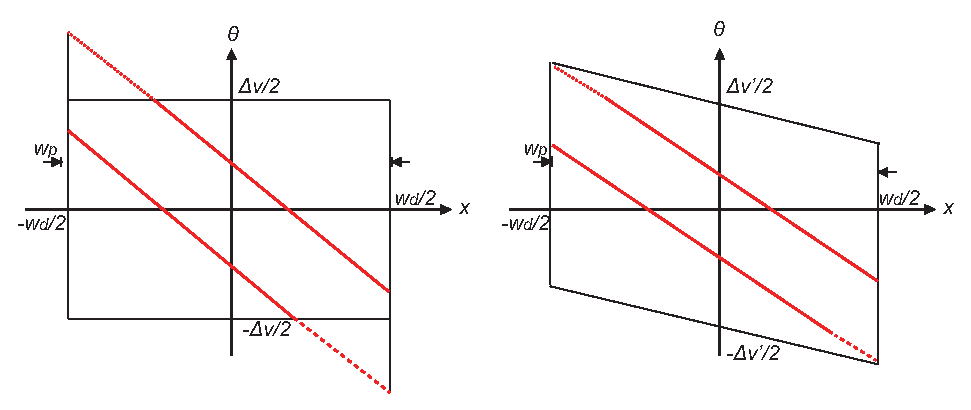
\includegraphics[width=0.95\linewidth]{images/CrossTalk.eps}
	    \end{center}
	\caption{Ray space diagram of display and eye. Left: Display with cross-talk; the dashed line corresponds to rays that are not captured by the display. Right: Pre-sheared display that takes oblique angled rays into consideration in order to avoid cross-talk.}
\label{fig:crosstalkDisplay}
\end{figure}

\begin{figure}
    \begin{center}
        \fbox{\rule{0pt}{2in} \rule{.45\linewidth}{0pt}}
    \end{center}
    \caption{Ray-space diagrams for higher-order aberration will appear here}
    \label{fig:rayspace_highorderaberration}
\end{figure}

